% Generated by experiments/paper/fig_transfer.py; do not edit.
\begin{figure*}[t]
\centering
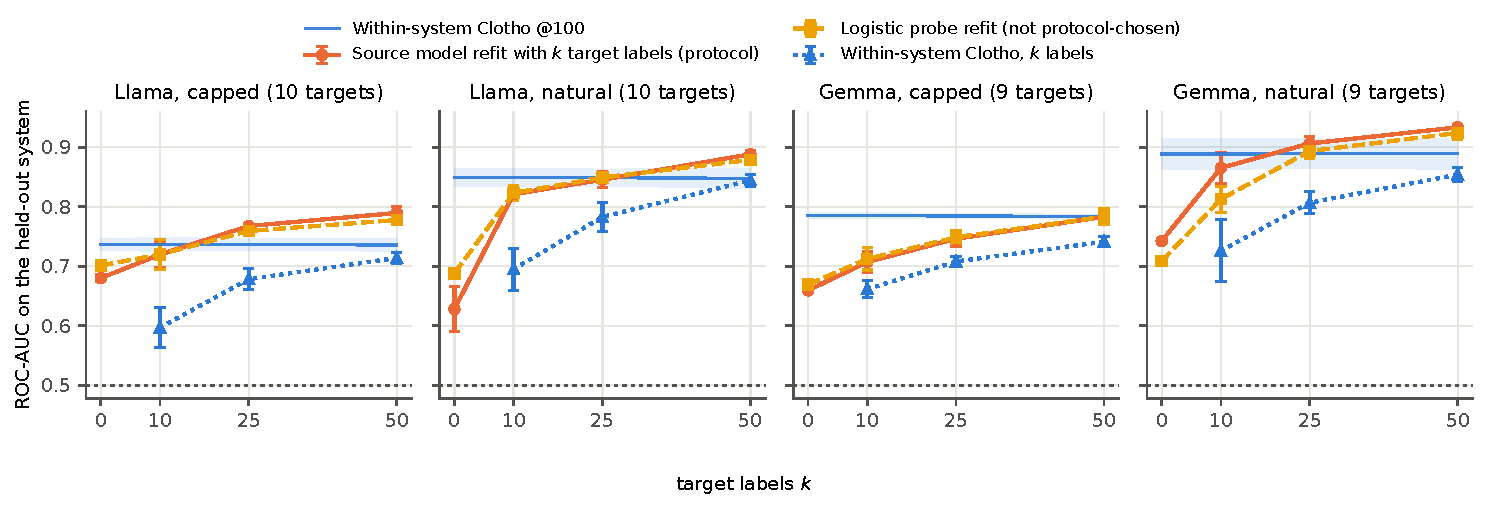
\includegraphics[width=\textwidth]{figures/transfer.pdf}
\caption{Failure prediction on a new log system (leave-one-system-out; held-out targets only, i.e. not HDFS, Spark or Linux, which chose every hyperparameter). Source model: trained on the pass/fail labels of all other systems (protocol-chosen: MLP probe for Llama, logistic probe + generic log features for Gemma), refit with $k$ random target labels; the logistic probe is shown for comparison but was not the protocol's choice. Within-system Clotho is fitted on the same $k$ labels, or on its own 90 actively sampled labels (@100, band = $\pm$ std). At each $k$ all lines are scored on the same target inputs. Label from samples 5--9; ROC-AUC, mean $\pm$ std over 5 seeds of the macro mean over targets.}
\label{fig:transfer}
\end{figure*}
